\chapter{Исследовательский раздел}
%Должен быть текст
\section{Тесты}

Были подготовлены тесты для вычисления расстояний между следующими строками:
\begin{itemize}
	\item ''skat'' и ''kot'';
	\item ''skat'' и '''';
	\item '''' и ''kot'';
	\item '''' и '''';
	\item ''kot'' и ''kot'';
	\item ''ab'' и ''ba''.
\end{itemize}

Также на рисунках 4.1 - 4.6 представлены результаты работы программы.
\begin{figure}
	\center{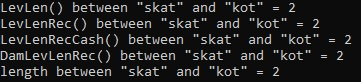
\includegraphics[scale=1]{inc/img/skat_kot}}
	\caption{Получившиеся расстояния между строками ''skat'' и ''kot''}
	\center{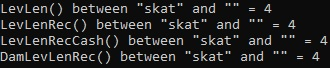
\includegraphics[scale=1]{inc/img/skat_}}
	\caption{Получившиеся расстояния между строками ''skat'' и ''''}
\end{figure}
\begin{figure}
	\center{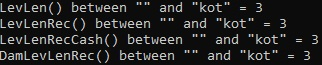
\includegraphics[scale=1]{inc/img/_kot}}
	\caption{Получившиеся расстояния между строками '''' и ''kot''}
	\center{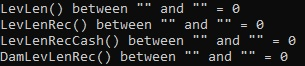
\includegraphics[scale=1]{inc/img/_}}
	\caption{Получившиеся расстояния между строками '''' и ''''}
	\center{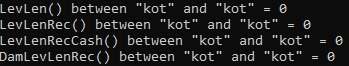
\includegraphics[scale=1]{inc/img/kot_kot}}
	\caption{Получившиеся расстояния между строками ''kot'' и ''kot''}
	\center{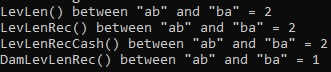
\includegraphics[scale=1]{inc/img/ab_ba}}
	\caption{Получившиеся расстояния между строками ''ab'' и ''ba''}
\end{figure}

\newpage
Как видно по рисункам, ответы сошлись с ожидаемым результатом, следовательно программа работает верно.

\section{Сравнительный анализ времени выполнения алгоритмов}
На графиках представленных ниже (рисунки 4.7-4.9), изображены зависимости времени выполнения алгоримов от длин слов, между которыми считались расстояния:

\begin{figure}
	\begin{tikzpicture}
		\begin{axis}[
			%title={Зависимость времени выполнения алгоритмов LenLev() и LenLevRecCash() от длины слов},
			xlabel={Длина слов, симв.},
			ylabel={Время выполнения, сек.},
			xtick={10,20,30,40,50},
			legend pos=north west,
			ymajorgrids=true,
			grid style=dashed,
			width = 400
			]
			
			\addplot[
			color=blue,
			mark=square,
			]
			coordinates {
				(10,5e-06)(20,1.31255e-05)(30,2.5e-05)(40,4e-05)(50,5.625e-05)
			};
			\addlegendentry{LevLen()}
			
			
			\addplot[
			color=red,
			mark=square,
			]
			coordinates {
				(10,0.000140625)(20,0.0015625)(30,0.0078125)(40,0.025)(50,0.0625)
			};
			\addlegendentry{LevLenRecCash()}
			
		\end{axis}
	\end{tikzpicture}
	\caption{Зависимость времени выполнения алгоритмов LenLev() и LenLevRecCash() от длины слов}
\end{figure}

\begin{figure}
	\begin{tikzpicture}
		\begin{axis}[
			%title={График зависимости времени выполнения алгоритмов LenLevRec() и LenLevRecCash() от длины слов},
			xlabel={Длина слов, симв.},
			ylabel={Время выполнения, сек.},
			xtick={6,7,8,9,10},
			legend pos=north west,
			ymajorgrids=true,
			grid style=dashed,
			width = 400
			]
			
			\addplot[
			color=blue,
			mark=square,
			]
			coordinates {
				(6,0.0018125)(7,0.01)(8,0.053125)(9,0.28125)(10,1.625)
			};
			\addlegendentry{LevLenRec()}
			
			
			\addplot[
			color=red,
			mark=square,
			]
			coordinates {
				(6,3.125e-05)(7,4.6875e-05)(8,6.25e-05)(9,0.000109375)(10,0.000140625)
			};
			\addlegendentry{LevLenRecCash()}
			
		\end{axis}
	\end{tikzpicture}
	\caption{Зависимость времени выполнения алгоритмов LenLevRec() и LenLevRecCash() от длины слов}
\end{figure}

\begin{figure}
	\begin{tikzpicture}
		\begin{axis}[
			%title={График зависимости времени выполнения алгоритмов LenLevRec() и 	DamLenLevRec() от длины слов},
			xlabel={Длина слов, симв.},
			ylabel={Время выполнения, сек.},
			xtick={6,7,8,9,10},
			legend pos=north west,
			ymajorgrids=true,
			grid style=dashed,
			width = 400
			]
			
			\addplot[
			color=blue,
			mark=square,
			]
			coordinates {
				(6,0.0018125)(7,0.01)(8,0.053125)(9,0.28125)(10,1.625)
			};
			\addlegendentry{LevLenRec()}
			
			
			\addplot[
			color=red,
			mark=square,
			]
			coordinates {
				(6,0.0018125)(7,0.009375)(8,0.053125)(9,0.296875)(10,1.625)
			};
			\addlegendentry{DamLenLevRec()}
			
		\end{axis}
	\end{tikzpicture}
	\caption{Зависимость времени выполнения алгоритмов LenLevRec() и DamLenLevRec() от длины слов}
\end{figure}

\newpage
Проанализировав графики, приходим к выводу, что самым быстрым алгоритмом является обычный (матричный) Левенштейн. А самыми медленными рекурсивные алгоритмы без кэширования.

\newpage
\section{Сравнительный анализ времени выполнения алгоритмов}
На рисунках 4.10 - 4.13 предсатвлены результаты оценки памяти алгоритмов, с помощью valgrind.

\begin{figure}[h]
	\center{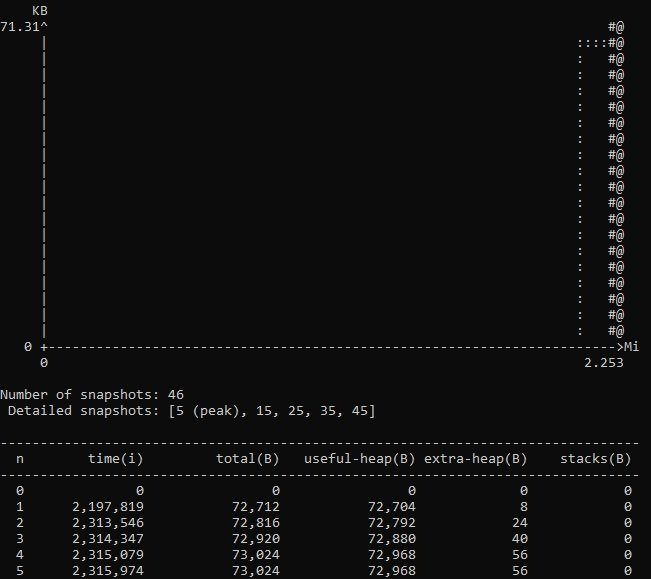
\includegraphics[scale=1]{inc/img/LevLenMemory}}
	\caption{Оценка памяти алгоритма LevLen()}
\end{figure}

\begin{figure}
	\center{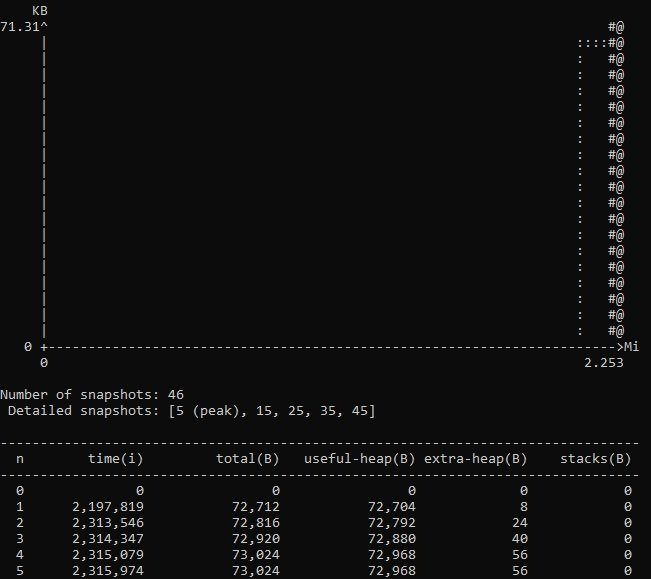
\includegraphics[scale=1]{inc/img/LevLenRecMemory}}
	\caption{Оценка памяти алгоритма LevLenRec()}
\end{figure}

\begin{figure}
	\center{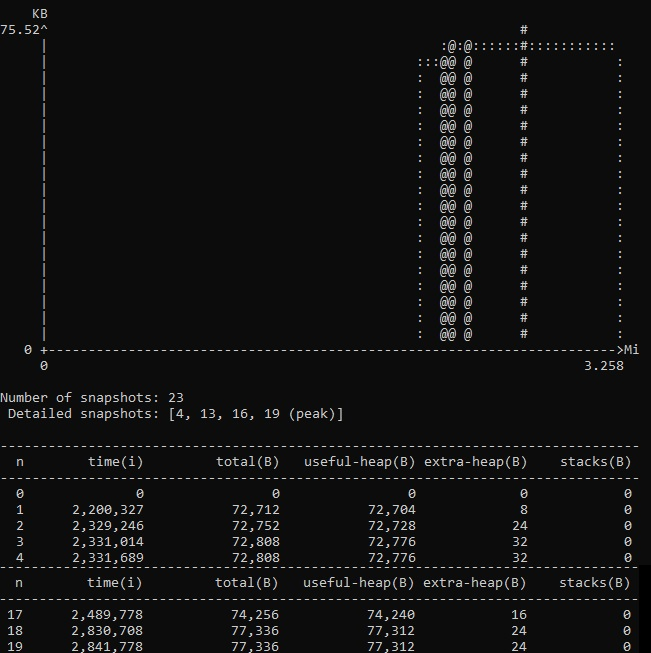
\includegraphics[scale=1]{inc/img/LevLenRecCashMemory}}
	\caption{Оценка памяти алгоритма LevLenRecCash()}
\end{figure}

\begin{figure}
	\center{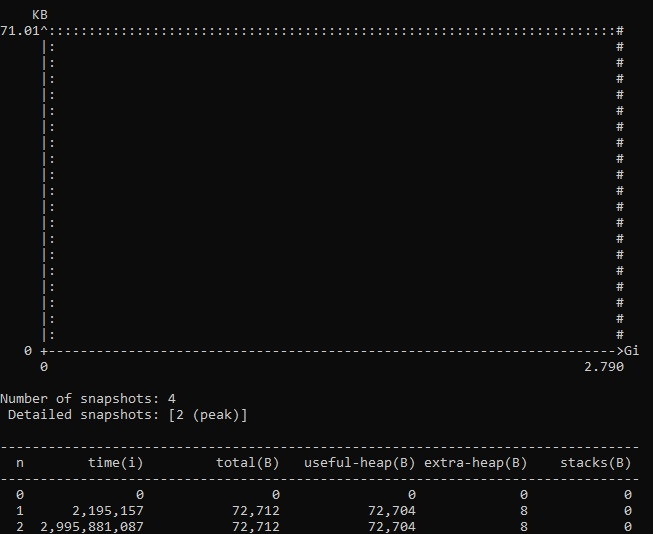
\includegraphics[scale=1]{inc/img/DamLevLenRecMemory}}
	\caption{Оценка памяти алгоритма DamLevLenRec()}
\end{figure}

\newpage
Судя по результатам меньше всего памяти нужно рекусривным алгоритмам, а больше всего алгоритму с кэшированием.

\section{Вывод}
По итогу иследования выяснилось, что разработанная программа работает верно. Кроме этого, смотря на время выполнения и используемую память каждого алгоритма, логично сделать вывод, что наиболее выгодный по использованию данных ресурсов, является обычный (матричный) Левенштейн.